\usetikzlibrary{arrows}
\begin{center}
    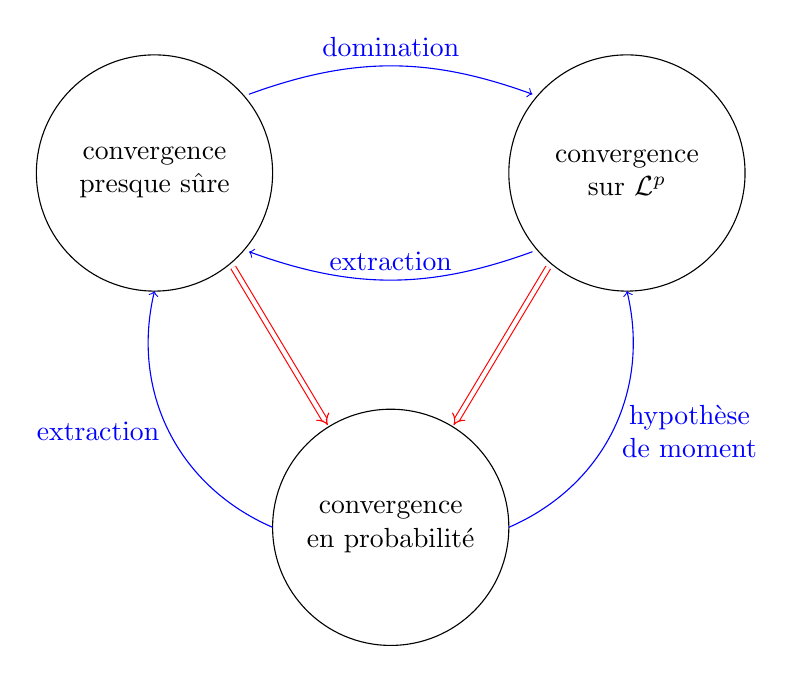
\begin{tikzpicture}[
        implies/.style={double equal sign distance, -implies},
        every node/.style={align=center}
    ]
        % Define the circle centers with labels
        \node (c1) at (-3, 2) {convergence\\presque sûre};
        \node (c2) at (3, 2) {convergence\\sur $\mathcal{L}^p$};
        \node (c3) at (0, -2.5) {convergence\\en probabilité};
        
        % Draw bigger circles around the centers
        \draw (c1) circle (1.5);
        \draw (c2) circle (1.5);
        \draw (c3) circle (1.5);
        
        % Red implication arrows (double lined) from top to bottom - now straight
        \draw[-implies, double equal sign distance, red] (-2, 0.8) -- (-0.8, -1.2);
        \draw[-implies, double equal sign distance, red] (2, 0.8) -- (0.8, -1.2);
        
        % Blue curved arrows between sets
        \draw[<-, blue] (-1.8, 1) to[bend right=20] node[above] {extraction} (1.8, 1);
        
        % Top extraction arrow now lower, mirroring the domination arrow
        \draw[<-, blue] (1.8, 3) to[bend right=20] node[above] {domination} (-1.8, 3);
        
        % Bottom arrows now start from circle sides
        \draw[->, blue] (-1.5, -2.5) to[bend left=40] node[left] {extraction} (-3, 0.5);
        
        \draw[->, blue] (1.5, -2.5) to[bend right=40] node[right] {hypothèse\\de moment} (3, 0.5);
    \end{tikzpicture}
\end{center}